\documentclass[11pt,a4paper]{article}

\usepackage{../../templates/style}

\begin{document}

\begin{problem}{Treasure}{standard input}{standard output}{1 second}{64 megabytes}

ในการเดินทางผจญภัยเพื่อค้นหาขุมทรัพย์ จะมีการใช้แผนที่ซึ่งเป็นสิ่งจำเป็นในการเดินทางเพื่อบอกทิศทางและระยะทางนำไปสู่ขุมทรัพย์ โดยสำหรับทิศทางจะใช้สัญลักษณ์ดังนี้
\begin{itemize}

\item \textbf{N }แทน ทิศเหนือ
\item \textbf{NE} แทน ทิศตะวันออกเฉียงเหนือ
\item \textbf{E} แทน ทิศตะวันออก
\item \textbf{SE} แทน ทิศตะวันออกเฉียงใต้
\item \textbf{S} แทน ทิศใต้
\item \textbf{SW} แทน ทิศตะวันตกเฉียงใต้
\item \textbf{W} แทน ทิศตะวันตก
\item \textbf{NW} แทน ทิศตะวันตกเฉียงเหนือ
\end{itemize}

สูตรในการหาระยะทางของตำแหน่งพิกัด และตำแหน่งพิกัด คำนวณได้ดังนี้
$$d(p_1,p_2) = \sqrt{(x_1-x_2)^2 + (y_1 - y_2)^2}$$
กำหนดให้การเดินทางเริ่มต้นที่พิกัด $(0, 0)$
\bigskip

\textbf{ตัวอย่าง}

\textbf{5SE} หมายถึงเดินทางไปทิศตะวันออกเฉียงใต้ $5$ หน่วย\\ \textbf{3N 1E 1N 3E 2S 1W} หมายถึงการเดินทางแสดงดังรูปที่ 1

\begin{figure}[h]
\centering
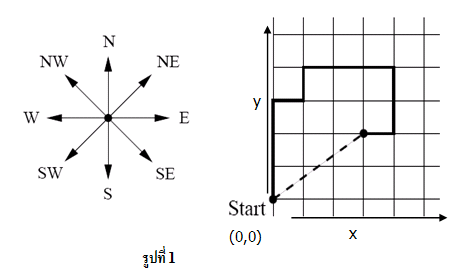
\includegraphics[width=0.6\textwidth]{../latex/img/1016/1016-2.png}
\end{figure}

\underline{\textbf{โจทย์}}  จงเขียนโปรแกรมเพื่อคำนวณหาพิกัดของขุมทรัพย์ $(x, y)$ และหาระยะห่างระหว่างจุดเริ่มต้น $(0,0)$ ไปยังพิกัดของขุมทรัพย์

\InputFile

\textbf{มีบรรทัดเดียว} รับระยะทางและทิศทางการเดินทาง $n$ ชุด $(1\leq n\leq 500)$ แต่ละชุดคั่นด้วยช่องว่างหนึ่งช่อง ในแต่ละชุดประกอบด้วยจำนวนเต็มบวก $k$ $(1\leq k\leq 999)$ เพื่อบอกระยะทาง และตัวอักษรหนึ่งหรือสองตัวเพื่อบอกทิศทาง ข้อมูลชุดสุดท้ายจะมีเฉพาะตัวอักขระ "*" เพื่อบอกการสิ้นสุดของชุดข้อมูล

\OutputFile

\textbf{บรรทัดแรก} ให้แสดงพิกัดของขุมทรัพย์ โดยแสดงเป็นลำดับตัวเลขของแกน x และแกน y ทศนิยม 3 ตำแหน่ง โดยคั่นข้อมูลด้วยช่องว่างหนึ่งช่อง

\textbf{บรรทัดที่สอง} ให้บอกระยะห่างจากจุดเริ่มต้น (0,0) ไปยังพิกัดของขุมทรัพย์ (x, y) เป็นตัวเลขซึ่งมีจุดทศนิยม 3 ตำแหน่ง

\Examples

\begin{example}
\exmp{3N 1E 1N 3E 2S 1W *}{3.000 2.000
3.606}%
\end{example}

\Note 

มีข้อแนะนำในการทำโจทย์ข้อนี้ ดังต่อไปนี้
\begin{enumerate}

\item ให้ใช้ ”\%.3f” เป็นรูปแบบของการแสดงผลเมื่อใช้คำสั่ง printf
\item เพื่อความแม่นยำในการคำนวณให้ประกาศตัวแปรด้วยแบบ double แทนการใช้ float
\end{enumerate}

\Source

การแข่งขันคอมพิวเตอร์โอลิมปิก สอวน. ครั้งที่ 3 มหาวิทยาลัยขอนแก่น

\end{problem}

\end{document}